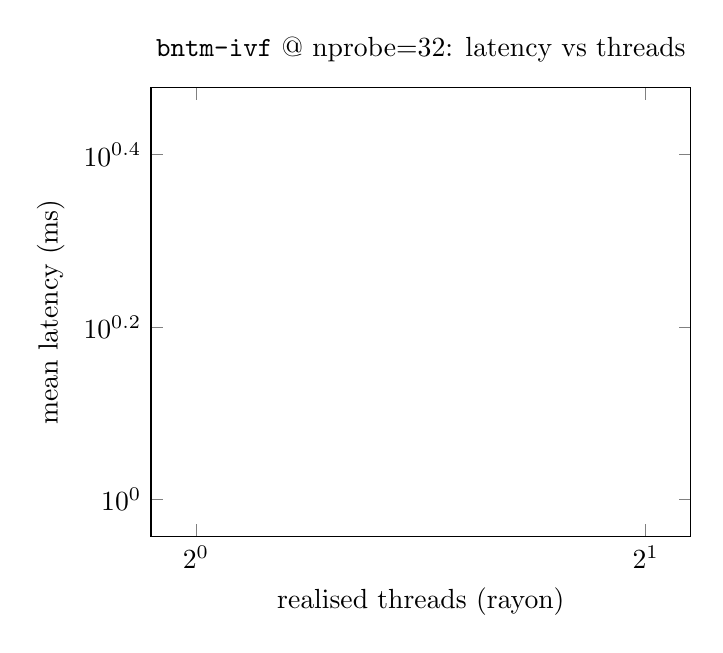
\begin{tikzpicture}
  \begin{axis}[
    xmode=log, log basis x=2, ymode=log,
    xlabel={realised threads (rayon)},
    ylabel={mean latency (ms)},
    title={\texttt{bntm-ivf} @ nprobe=32: latency vs threads},
    legend style={
      at={(0.02,0.02)}, anchor=south west,
      draw=none, fill=white, fill opacity=0.85, text opacity=1,
      font=\sffamily\footnotesize,
    },
    legend columns=1,
  ]
    \foreach \slug/\dlabel in \canonicalSeries {%
      \IfFileExists{\datadir/03-parallel-scaling-bntm-ivf-nprobe-32-\slug.tsv}{%
        \edef\xtemp{%
          \noexpand\addplot+ table[x=threads, y=latency_ms]
            {\datadir/03-parallel-scaling-bntm-ivf-nprobe-32-\slug.tsv};%
          \noexpand\addlegendentry{\dlabel}%
        }\xtemp
      }{}%
    }
  \end{axis}
\end{tikzpicture}
